\documentclass[tikz,border=10pt]{standalone}
\usetikzlibrary{calc}
\begin{document}
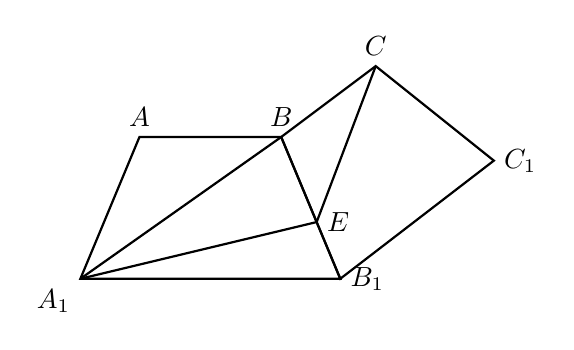
\begin{tikzpicture}[scale=1.5,thick,>=stealth]
    % 定义关键坐标点 (模拟透视坐标)
    \coordinate (A)  at (0, 1.2);
    \coordinate (B)  at (1.2, 1.2);
    \coordinate (C)  at (2, 1.8);
    \coordinate (A1) at (-0.5, 0);
    \coordinate (B1) at (1.7, 0);
    \coordinate (C1) at (3.0, 1.0);
    
    % 计算点 E: 在线段 B-B1 上取一点
    % 使用 barycentric coordinates 计算 E (例如位于 BB1 的 0.6 处)
    \coordinate (E) at ($(B)!0.6!(B1)$);

    % 绘制四边形 ABB1A1
    \draw (A) -- (B) -- (B1) -- (A1) -- cycle;
    
    % 绘制四边形 BCC1B1
    \draw (B) -- (C) -- (C1) -- (B1) -- cycle;
    
    % 绘制内部辅助线
    \draw (A1) -- (B);
    \draw (A1) -- (E);
    \draw (C) -- (E);

    % 标注顶点
    \node[above] at (A) {$A$};
    \node[above] at (B) {$B$};
    \node[above] at (C) {$C$};
    \node[below left] at (A1) {$A_1$};
    \node[right] at (B1) {$B_1$};
    \node[right] at (C1) {$C_1$};
    \node[right] at (E) {$E$};

\end{tikzpicture}
\end{document}